%%%%%%%%%%%%%%%%%%%%%%%%%%%%%%%%%%%%%%%%%%%%%%%%%%%%%%%%%%%%%%%%%%%%
%-------------------------------------------------------------------
% Selected Approach
%-------------------------------------------------------------------
%%%%%%%%%%%%%%%%%%%%%%%%%%%%%%%%%%%%%%%%%%%%%%%%%%%%%%%%%%%%%%%%%%%%
\selectlanguage{british}
\chapter{Selected Approach}
\label{toc:selected}

This chapter presents the approach selected for carrying out the 
project described in chapter~\ref{toc:project}. First, the selected 
open-source solutions used in the project are listed. Secondly, an 
overview of the the architecture designed for the new system is 
presented. Thirdly, the agile methodologies that were chosen for the 
project are given. After that, the project team is introduced. 
Finally, the methods used for evaluating the project are presented.


%%%%%%%%%%%%%%%%%%%%%%%%%%%%%%%%%%%%%%%%%%%%%%%%%%%%%%%%%%%%%%%%%%%%
% Selected Open-Source Solutions
%%%%%%%%%%%%%%%%%%%%%%%%%%%%%%%%%%%%%%%%%%%%%%%%%%%%%%%%%%%%%%%%%%%%
\section{Selected Open-Source Solutions}
\label{toc:selected:oss}

To minimise the amount of code needed to implement in-house, all the 
open-source solutions introduced in chapter~\ref{toc:oss} were 
selected for use in the project. The solutions and their usage in this 
project are listed below.

\begin{description}

\item[Apache Struts] Struts was selected as the web framework to be 
used in the project. In the new system, Struts is responsible for 
managing the dynamic web page creation and processing the input sent 
by the user. JavaServer Pages will be used as the view components that 
will render the actual \abbrev{XHTML} content.

\item[Spring Framework] Spring was selected as the application context 
that creates and configures most of the objects used in the system. 
Although Struts has its own way of creating the required action 
objects, Spring and Struts can and will be integrated so that the 
Struts action objects are under Spring control.

\item[Hibernate] Hibernate was selected to handle data persisting to 
database. All persisted objects in the system are annotated with 
special Hibernate metadata, so that they can be automatically stored 
to and retrieved from the database. Spring is configured to select 
Hibernate as the data source for the application.

\item[XDoclet] XDoclet was selected for automatic artifact generation. 
In this project, XDoclet is configured to automatically generate 
Hibernate mapping data and parts of Struts and Spring configuration 
files from XDoclet tags written in Java source code files.

\item[Eclipse] Eclipse was selected to be used for developing the 
system. The source code supporting tools in Eclipse's Java Development 
Toolkit have been found useful in previous projects.

\item[Apache Maven] Maven was selected to handle the building of the 
system. Especially the idea of not having to specify the project paths 
and Java classpaths was seen as an appealing idea.

\item[Subversion] Subversion was chosen as the version control system 
for the project. Subversion was selected over the tradition 
\abbrev{CVS} since it has been developed as a replacement for 
\abbrev{CVS} and it addresses some of the shortcomings of \abbrev{CVS}.

\end{description}


%%%%%%%%%%%%%%%%%%%%%%%%%%%%%%%%%%%%%%%%%%%%%%%%%%%%%%%%%%%%%%%%%%%%
% System Architecture Overview
%%%%%%%%%%%%%%%%%%%%%%%%%%%%%%%%%%%%%%%%%%%%%%%%%%%%%%%%%%%%%%%%%%%%
\section{System Architecture Overview}
\label{toc:selected:architecture}

Since the current system is a standard web application that is used 
with a normal web browser, it was decided that the new system will 
also be a normal web application. The three-tier model, which was 
described in section~\ref{toc:webdevel:threetier}, was selected as the 
basis for the implementation.

The most important components of the designed architecture are shown 
in figure~\ref{fig:architecture}. The lines connecting the components 
describe the response handling path of a standard query initiated from 
the user's browser. The numbers in the figure correspond to the steps 
described below.

\begin{figure}
\begin{center}
  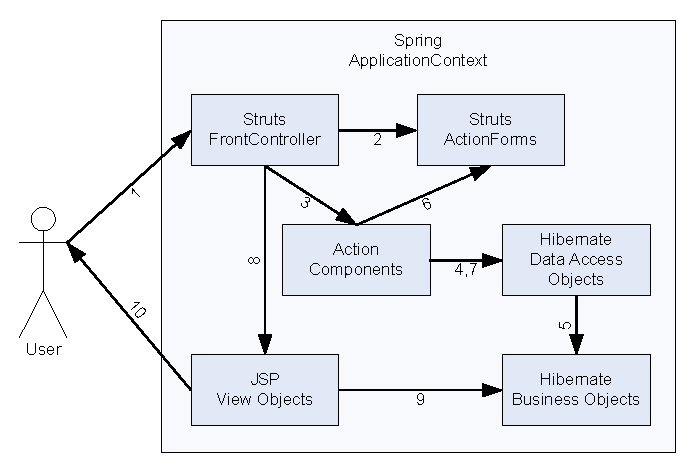
\epsfig{file=images/architecture.eps, width=100mm}
  \caption{System Architecture}
  \label{fig:architecture}
\end{center}
\end{figure}

\begin{enumerate}

  \item User initiates a request by clicking on a link or by posting a 
  form in the system. The request is received by the Struts 
  \code{FrontController}.
  
  \item The \code{FrontController} generates or populates the Struts 
  \code{ActionForm} associated with the request from the request data. 
  Query parameters are automatically parsed and inserted into the form.
  
  \item The \code{FrontController} selects the proper 
  application-specific action component, and passes control to it. The 
  prefilled \code{ActionForm} is passed to the action as a parameter.
  
  \item The action loads required data from data access objects, which 
  are implemented using Hibernate.
  
  \item The data access objects automatically load the required 
  business objects from the database, and return them to the action 
  component.
  
  \item The action component performs the required actions on the 
  business objects as requested by the request parameters and 
  \code{ActionForms}. Data from \code{ActionForms} is transferred to 
  the business objects.
  
  \item The action component persists the modified business objects by 
  using the data access objects, and returns control to the Struts 
  \code{FrontController}.
  
  \item The \code{FrontController} selects the proper view to show to 
  the user based on the return value of the action component. The 
  action component can indicate whether the action was processed 
  successfully, or if an error page should be shown.
  
  \item The selected \abbrev{JSP} page is rendered by using the 
  retrieved business objects as data sources. The design was 
  simplified by allowing the business objects to work as data transfer 
  objects (and as helper objects in the front controller design 
  pattern).
  
  \item The rendered page is sent back to the user's browser.
  
\end{enumerate}

The architecture for the web components is largely dictated by Struts. 
Struts implements the model-view-controller design pattern with the 
\code{FrontController} and actions working as the controller, the 
\abbrev{JSP} pages as the view, and the application-specific business 
objects and data access objects as the model. The front controller 
design pattern is also realised with the \code{FrontController} 
provided by Struts working as the controller and dispatcher, the 
\abbrev{JSP} pages as the view, and the business objects as the 
helpers.

The business objects in the system are initialised using the Spring 
application context. Spring configures the objects using the inversion 
of control design pattern. The mappings between the objects are 
written to a configuration file, and Spring is responsible for setting 
up the links between the objects via setter injection.

The database mappings in the database tier are configured with the 
object/relational mapping provided by Hibernate. Special Hibernate 
metadata is annotated in the business object Java code files.


%%%%%%%%%%%%%%%%%%%%%%%%%%%%%%%%%%%%%%%%%%%%%%%%%%%%%%%%%%%%%%%%%%%%
% Selected Agile Development Methods
%%%%%%%%%%%%%%%%%%%%%%%%%%%%%%%%%%%%%%%%%%%%%%%%%%%%%%%%%%%%%%%%%%%%
\section{Selected Agile Development Methods}
\label{toc:selected:agile}

This section lists the agile software development methods selected for 
use in the project, and presents the criteria for selecting them. For 
the project, methods from both Extreme Programming and Scrum were 
selected. As suggested in section~\ref{toc:agile:adopt}, it is better 
to only select a few methods for use instead of trying to tackle all 
the methods given in an agile methodology at once.


% XP Practices
% ------------
\subsection{XP Practices}
\label{toc:selected:agile:xp}

For developing the software, a subset of six \abbrev{XP} practices was 
selected. The selected practices are listed below alongside with 
justification for their selection.

\begin{description}

\item[Short Releases] Without short releases the design for the system 
needs to be finalised before the start of the implementation phase. 
With short releases, it is possible to leave some implementation 
details a bit unclear at the beginning of the project and iterate them 
with the customer between the releases.

\item[Refactoring] Since some of the requirements are likely to change
somewhat during the implementation phase, the code needs to be
refactored from time to time.

\item[Testing] Testing is required to make refactoring possible. 
Testing was also selected because it has been seen to produce better 
quality, as discussed in section~\ref{toc:agile:xp:practices}, and
because it has been identified as the most important \abbrev{XP}
practice. 

\item[Collective Ownership] Collective code ownership is another 
requirement for refactoring. To be able to refactor efficiently, 
developers need to be able to modify every part of the codebase.

\item[Simple Design] Since refactoring is expected to happen 
frequently, the design should be kept simple. Simple designs are more 
easily changed and are less error-prone.

\item[Coding Standards] Coding standards were also chosen to support 
refactoring. For this project, coding standards mean indentation rules 
as well as rules about where different information should be placed.

\end{description}

This subset of \abbrev{XP} was seen to be small enough to be easy to 
adapt to. The selected practices were chosen so that they support each 
other as much as possible. For example, the subset would not be 
functional if refactoring or testing was left out.

% Scrum Practices
% ---------------
\subsection{Scrum Practices}
\label{toc:selected:agile:scrum}

Although some authors suggest adopting agile methods only a few at a 
time, they are most often talking about \abbrev{XP} practices or other 
development practices. When talking about Scrum, it is suggested that 
Scrum should be adopted all at once. However, it was decided that the 
Scrum review, meeting and the practices between sprints will be left 
out because the project is small. The estimated size for the project 
is only a couple of sprints. The selected practices are listed below 
with justifications for their selection.

\begin{description}

\item[Product Backlog] The product backlog was selected to function as 
the requirement repository, which contains all the currently known 
tasks. The backlog will be updated whenever a new requirement is 
received or when additional information for an existing requirement is 
available.

\item[Effort Estimation] The client required an approximate effort 
estimation for the entire project before the start of the 
implementation phase. The initial estimates were selected as the 
starting point for the project effort estimates, even though this does 
not exactly adhere to Scrum ideology. In pure Scrum, only the 
requirements for the next sprint should be estimated.

\item[Sprint] To support the \abbrev{XP} short releases practice, the
Scrum sprints were selected as the short iterations.

\item[Daily Scrum Meeting] The daily Scrum meetings were selected as
the main team organisational activity. Since both the project and the
project team is small, this meeting was seen as an adequate way of
keeping everyone up-to-date with the current project status.

\end{description}

For this small project, this adoption of the Scrum process was seen as 
an adequate set of project management practices. The practices were
selected so that they support the \abbrev{XP} practices selected in
section~\ref{toc:selected:agile:xp}.


%%%%%%%%%%%%%%%%%%%%%%%%%%%%%%%%%%%%%%%%%%%%%%%%%%%%%%%%%%%%%%%%%%%%
% Project Team
%%%%%%%%%%%%%%%%%%%%%%%%%%%%%%%%%%%%%%%%%%%%%%%%%%%%%%%%%%%%%%%%%%%%
\section{Project Team}
\label{toc:selected:team}

The development team for the project consists of three developers from 
\finnish{HiQ Softplan Oy}. Two of them are currently writing their 
Master's Theses, and one is a graduated Master of Science. All three 
have over five years of work experience behind them in the software 
engineering field.

The team members possess a good knowledge of Java frameworks, but they 
are not intimately familiar with all of the selected solutions. 
Furthermore, the team members have not been working on a project that 
uses agile methodologies to any greater extent before, but have 
studied the theories behind the methodologies.


%%%%%%%%%%%%%%%%%%%%%%%%%%%%%%%%%%%%%%%%%%%%%%%%%%%%%%%%%%%%%%%%%%%%
% Evaluation of the Project
%%%%%%%%%%%%%%%%%%%%%%%%%%%%%%%%%%%%%%%%%%%%%%%%%%%%%%%%%%%%%%%%%%%%
\section{Evaluation of the Project}
\label{toc:selected:evaluation}

To evaluate the outcome of the project, some concrete measurements 
need to be made. This section lists the methods selected to evaluate 
both the outcome of the project and the project itself. To achieve 
this, the \abbrev{CK} metrics were selected to measure the developed 
software, and the \abbrev{XP} Evaluation Framework was selected to 
evaluate the adoption of the \abbrev{XP} practices.


% Software Quality
% ----------------
\subsection{Software Quality}
\label{toc:selected:evaluation:quality}

The Chidamber-Kemerer metrics suite (see 
section~\ref{toc:evaluation:ck}) was selected for measuring the 
quality of the produced software. All the six metrics in the 
\abbrev{CK} suite will be measured with the open-source tool 
AOPMetrics \citep{aopmetrics} at the end of the project. AOPMetrics 
supports measuring both AspectJ and normal Java code. Thus the metrics 
used in it are named a bit differently than the standard \abbrev{CK} 
metrics, but they are equivalent. As AOPMetrics is a free open-source 
tool, it was selected for use in this project.

The problem with measurements is that they are not useful by 
themselves, but require a comparison point to provide concrete 
feedback. Unfortunately the source codes for the original software are 
not available. However, \cite{oodmetrics} and \cite{ckanalysis} 
provide a total of four measurements of different software systems. 
These shall be used as a comparison point in evaluating the obtained 
\abbrev{CK} metric values.


% Agile Practice Adoption
% -----------------------
\subsection{Agile Method Adoption}
\label{toc:selected:evaluation:agileadoption}

The \abbrev{XP} Evaluation Framework (see 
section~\ref{toc:evaluation:xpef}) will be used to evaluate the 
adoption of agile practices in the project. Of the three parts of 
\abbrev{XP-EF}, only the \abbrev{XP} adherence metrics will be 
measured. In addition, only the practices that were taken into use 
will be evaluated. This was selected as the approach because the 
\abbrev{XP} context factors are mainly useful for comparison 
purposes between multiple projects and the \abbrev{XP} outcome 
measures contain very few other metrics than the \abbrev{CK} metrics 
that could be measured with the selected \abbrev{XP} practices.

The questionnaire used for the \abbrev{XP} adherence metrics 
subjective measures is shown in appendix~\ref{toc:appendix:shodan}. 
The questions will be asked from all team members, and the average 
percentages derived from the answers will be used to subjectively 
measure the adoption of the corresponding practices. The weights shown 
in figure~\ref{fig:xpweights} are used to obtain a weighted average of 
the answers. This value tells the overall adoption of \abbrev{XP} 
practices. The figure was adopted from \citep{xpexplained} by removing 
the practices that were not taken into use in this project. The 
weights of the practices were obtained by calculating the amount of 
other practices a single practice is connected to. In addition, the 
objective measures listed in \citep{xpevaluationfw} will be measured 
for the practices that were taken into use. The selected metrics are 
shown in appendix~\ref{toc:appendix:adherence}.

\begin{figure}
\begin{center}
  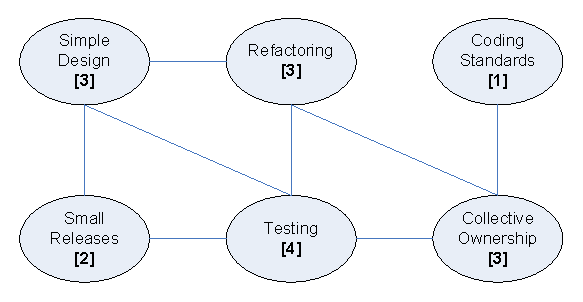
\epsfig{file=images/xppractices.eps, width=80mm}
  \caption{\abbrev{XP} Practice Weights}
  \label{fig:xpweights}
\end{center}
\end{figure}


%%%%%%%%%%%%%%%%%%%%%%%%%%%%%%%%%%%%%%%%%%%%%%%%%%%%%%%%%%%%%%%%%%%%
% Summary
%%%%%%%%%%%%%%%%%%%%%%%%%%%%%%%%%%%%%%%%%%%%%%%%%%%%%%%%%%%%%%%%%%%%
\section{Summary}
\label{toc:selected:summary}

This chapter explained the approach selected to execute the project
described in chapter~\ref{toc:project}. The selected solutions and
methods were presented.

Section~\ref{toc:selected:oss} listed the open-source solutions 
selected for use in the project. All the solutions presented in 
section~\ref{toc:oss:selected} were selected for use in the project. 
The solutions were selected to both cover the architecture of the 
system and to provide support to the software development process.

In section~\ref{toc:selected:architecture}, an overview of the system 
architecture was given. The system architecture was largely dictated 
by the selected open-source frameworks, which is often the case. 
Because the developed application is a web application, Apache Struts 
defines the basic structure of the architecture.

After that, section~\ref{toc:selected:agile} described the agile 
practices selected for use in the project. A subset of both 
\abbrev{XP} and Scrum practices was adopted for the project. The 
practices were selected so that they support each other as much as 
possible.

In section~\ref{toc:selected:team}, the project team was introduced. 
The team consists of three experienced software developers, ready for 
their first agile project.

Finally, section~\ref{toc:selected:evaluation} presented the 
evaluation methods that will be used to measure and evaluate the 
project. The \abbrev{CK} metric suite was selected to measure the 
produced software, and the \abbrev{XP} adherence metrics of the 
\abbrev{XP} Evaluation Framework were selected to evaluate the 
adoption of \abbrev{XP} practices.
